\documentclass[12pt,a4paper]{article}
\usepackage[utf8]{inputenc}
\usepackage{graphicx}
\usepackage{geometry}
\usepackage{titlesec}
\usepackage{fancyhdr}
\usepackage{hyperref}
\usepackage{listings}
\usepackage{xcolor}
\usepackage{float}
\usepackage{caption}
\usepackage{subcaption}
\usepackage{tikz}
\usepackage{afterpage}

\geometry{margin=1in}
\pagestyle{fancy}
\fancyhf{}
\fancyhead[L]{\leftmark}
\fancyhead[R]{\thepage}
\renewcommand{\headrulewidth}{0.4pt}

% Section formatting
\titleformat{\section}
{\normalfont\Large\bfseries}{\thesection}{1em}{}
\titlespacing*{\section}{0pt}{20pt}{12pt}

\titleformat{\subsection}
{\normalfont\large\bfseries}{\thesubsection}{1em}{}
\titlespacing*{\subsection}{0pt}{12pt}{8pt}

% Code listing style
\lstset{
    basicstyle=\ttfamily\small,
    breaklines=true,
    frame=single,
    backgroundcolor=\color{gray!10}
}

% Hyperref setup
\hypersetup{
    colorlinks=true,
    linkcolor=blue,
    filecolor=magenta,
    urlcolor=cyan,
    pdftitle={Collaborative Whiteboard TCP Project Report},
    pdfauthor={Student Names}
}

\begin{document}

% Cover Page
\begin{titlepage}
    \thispagestyle{empty}
    \centering
    
    % Top section with logo and university info
    \vspace*{1cm}
    
    % Logo
    \includegraphics[width=3.5cm]{logo.png}\\[1cm]
    
    % University Name
    {\fontsize{22}{26}\selectfont \textbf{UNIVERSITY OF DHAKA}}\\[0.4cm]
    
    % Department Name
    {\fontsize{16}{20}\selectfont \textsc{Department Of Computer Science & Engineering}}\\[1.2cm]
    
    % Horizontal line
    \rule{\textwidth}{1.5pt}\\[0.8cm]
    
    % Course Name
    {\fontsize{15}{19}\selectfont \textbf{CSE-3111: Computer Networking Lab}}\\[1.5cm]
    
    % Project Title Box
    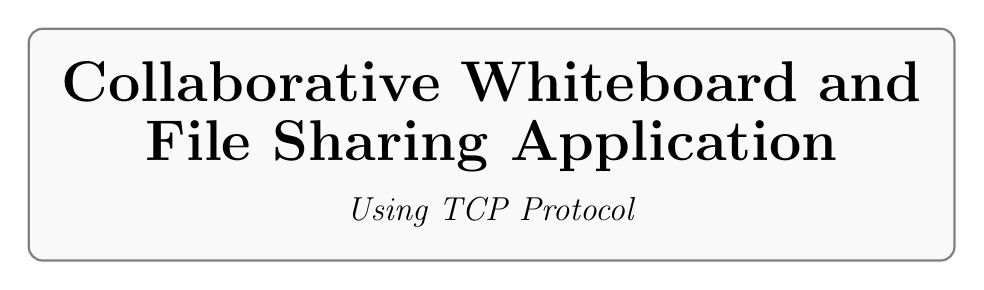
\begin{tikzpicture}
        \node[draw=black!50, thick, rounded corners=5pt, inner sep=12pt, fill=gray!5] {
            \begin{minipage}{0.9\textwidth}
                \centering
                {\fontsize{20}{24}\selectfont \textbf{Collaborative Whiteboard and}}\\[0.2cm]
                {\fontsize{20}{24}\selectfont \textbf{File Sharing Application}}\\[0.3cm]
                {\fontsize{13}{17}\selectfont \textit{Using TCP Protocol}}
            \end{minipage}
        };
    \end{tikzpicture}
    
    \vspace{2cm}
    
    % Information section - Instructors on left, Students on right
    \begin{minipage}{0.48\textwidth}
        \raggedright
        {\fontsize{13}{17}\selectfont \textbf{Instructors:}}\\[0.4cm]
        {\fontsize{11}{15}\selectfont 
        Dr. Shabbir Ahmed\\[0.15cm]
        Palash Roy\\[0.15cm]
        Ismat Rahman\\[0.15cm]
        Md. Mamun-or-Rashid}
    \end{minipage}
    \hfill
    \begin{minipage}{0.48\textwidth}
        \raggedright
        {\fontsize{13}{17}\selectfont \textbf{Students:}}\\[0.4cm]
        {\fontsize{11}{15}\selectfont 
        Roll 48 - Farhana Alam\\[0.15cm]
        Roll 16 - Ibna Afra Roza}
    \end{minipage}
    
    \vspace{2cm}
    
    % Bottom section with date
    \rule{\textwidth}{0.5pt}\\[0.4cm]
    {\fontsize{13}{17}\selectfont \textbf{\today}}
    
\end{titlepage}

% Table of Contents
\tableofcontents
\newpage
\listoffigures
\newpage

% Section 1: Overview
\section{Overview}
\label{sec:overview}

This project presents a comprehensive collaborative whiteboard and file sharing application built entirely using TCP protocol without any WebSocket dependencies. The system enables multiple users to interact in real-time through a shared whiteboard interface, integrated chat functionality, and secure file transfer capabilities. The application is designed to be cross-platform compatible, running seamlessly on Windows, macOS, and Linux operating systems.

The core architecture follows a client-server model where a central TCP server manages all client connections and coordinates message broadcasting. Each client maintains a persistent TCP connection to the server, enabling real-time synchronization of whiteboard drawings, chat messages, and file transfers across all connected participants.

The implementation leverages Java and JavaFX for the graphical user interface, ensuring a professional and consistent user experience across different platforms. The custom TCP protocol implementation demonstrates fundamental networking concepts including socket programming, reliable data transfer, and message framing.

% Section 2: Motivation
\section{Motivation}
\label{sec:motivation}

The motivation for developing this collaborative whiteboard application stems from the increasing need for real-time collaborative tools in educational and professional environments. Traditional whiteboard applications often rely on WebSocket protocols or cloud-based services, which introduce dependencies and potential latency issues.

By implementing a pure TCP-based solution, this project demonstrates a deeper understanding of low-level networking protocols and provides a foundation for understanding how modern collaborative applications function at the network layer. The project serves as a practical application of networking course concepts, including socket programming, protocol design, and reliable data transmission.

Additionally, the requirement to support multiple platforms without platform-specific code challenges the development of truly cross-platform network applications, making this project an excellent learning opportunity for understanding both networking and software engineering principles.

% Section 3: Problem Statement
\section{Problem Statement}
\label{sec:problem}

The primary problem addressed by this project is the development of a real-time collaborative whiteboard application that:

\begin{itemize}
    \item Enables multiple users to draw simultaneously on a shared canvas with real-time synchronization
    \item Provides a communication channel through integrated chat functionality
    \item Supports secure file sharing between connected clients
    \item Operates exclusively using TCP protocol without WebSocket dependencies
    \item Maintains consistent functionality and user interface across Windows, macOS, and Linux platforms
    \item Handles concurrent client connections efficiently through a centralized server architecture
    \item Preserves drawing history for newly connected clients to maintain session continuity
\end{itemize}

The challenge lies in designing a robust protocol that ensures reliable message delivery, handles network interruptions gracefully, and maintains state consistency across all connected clients while operating purely over TCP connections.

% Section 4: Design Goals and Objectives
\section{Design Goals and Objectives}
\label{sec:goals}

\section{Primary Objectives}

\begin{enumerate}
    \item \textbf{Real-time Collaboration:} Enable multiple users to interact simultaneously with immediate synchronization of all actions across all clients.
    
    \item \textbf{Reliable Communication:} Implement a robust TCP-based protocol ensuring message delivery and handling connection failures gracefully.
    
    \item \textbf{Cross-platform Compatibility:} Develop a single codebase that functions identically on Windows, macOS, and Linux without platform-specific modifications.
    
    \item \textbf{User Experience:} Provide an intuitive, professional interface with responsive drawing, clear chat display, and seamless file transfer capabilities.
    
    \item \textbf{Scalability:} Design the server architecture to handle multiple concurrent client connections efficiently.
\end{enumerate}

\section{Technical Objectives}

\begin{itemize}
    \item Implement custom TCP protocol with length-prefixed message framing
    \item Design thread-safe server architecture for concurrent client handling
    \item Develop efficient message broadcasting mechanisms
    \item Create state management system for whiteboard history preservation
    \item Implement targeted file transfer with recipient selection capabilities
\end{itemize}

% Section 5: Project Features
\section{Project Features}
\label{sec:features}

\section{Collaborative Whiteboard}

The whiteboard feature provides a shared canvas where all connected users can draw simultaneously. Key capabilities include:

\begin{itemize}
    \item Freehand drawing with customizable color selection
    \item Adjustable stroke width (1-15 pixels)
    \item Real-time stroke synchronization across all clients
    \item Board clearing functionality that affects all connected users
    \item Local save functionality to export whiteboard as PNG image
    \item Board snapshot sharing to distribute current state to all clients
\end{itemize}

\section{Integrated Chat System}

The chat system enables real-time text communication among all connected clients:

\begin{itemize}
    \item Broadcast messaging to all participants
    \item Message history preservation for newly connected clients
    \item Clear sender identification with "Me" label for own messages
    \item Server information messages for connection status updates
\end{itemize}

\section{File Sharing}

The file sharing feature allows users to send files to selected recipients:

\begin{itemize}
    \item Selective recipient targeting (single or multiple clients)
    \item Automatic file renaming with unique identifiers (e.g., \texttt{demo\_24343.txt})
    \item Base64 encoding for binary file transmission
    \item User notification upon file receipt with save location information
    \item Support for any file type and size
\end{itemize}

\section{Client Management}

The server maintains awareness of all connected clients:

\begin{itemize}
    \item Dynamic client list updates
    \item Unique client ID assignment
    \item Display name management
    \item Connection status monitoring
\end{itemize}

\section{TCP Congestion Control Visualization}

The application includes a comprehensive congestion control visualization feature:

\begin{itemize}
    \item \textbf{Algorithm Selection:} Toggle between TCP Tahoe and TCP Reno algorithms
    \item \textbf{Real-time Metrics:} Display current congestion window (cwnd), slow start threshold (ssthresh), round trip time (RTT), and current phase
    \item \textbf{Interactive Graph:} Live visualization of cwnd evolution over transmission rounds showing slow start, congestion avoidance, and recovery phases
    \item \textbf{Network Simulation:} Configurable packet loss rate (0-10\%) and network delay (0-200ms) for testing different network conditions
    \item \textbf{Activity Log:} Real-time log of congestion control events including phase transitions, timeouts, and fast retransmit events
    \item \textbf{Client-side Simulation:} Visualization layer that doesn't affect actual message transmission, maintaining backward compatibility
\end{itemize}

% Section 6: Block Diagram and Work Flow
\section{Block Diagram and Work Flow}
\label{sec:workflow}

\section{System Architecture}

The system follows a centralized client-server architecture as illustrated in Figure~\ref{fig:architecture}.

\begin{figure}[H]
    \centering
    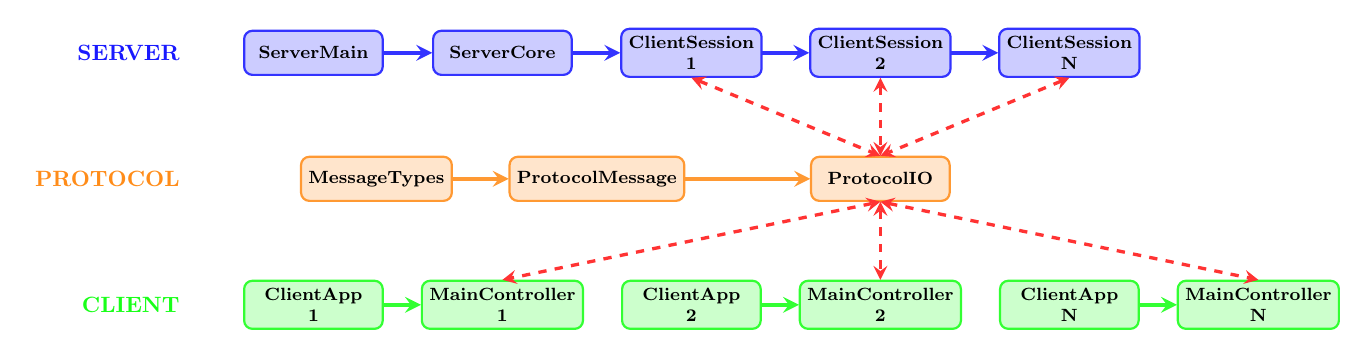
\begin{tikzpicture}[
        scale=0.80,
        transform shape,
        server/.style={rectangle, draw=blue!80, fill=blue!20, thick, minimum width=2.2cm, minimum height=0.7cm, text centered, font=\footnotesize\bfseries, rounded corners=3pt, align=center},
        client/.style={rectangle, draw=green!80, fill=green!20, thick, minimum width=2.2cm, minimum height=0.7cm, text centered, font=\footnotesize\bfseries, rounded corners=3pt, align=center},
        common/.style={rectangle, draw=orange!80, fill=orange!20, thick, minimum width=2.2cm, minimum height=0.7cm, text centered, font=\footnotesize\bfseries, rounded corners=3pt, align=center},
        arrow/.style={->, >=stealth, thick, line width=1.5pt},
        tcpArrow/.style={<->, >=stealth, dashed, thick, line width=1.2pt, color=red!80}
    ]
        
        % ========== SERVER LAYER (Top Row) ==========
        \node[server] (serverMain) at (1.5,4) {ServerMain};
        \node[server] (serverCore) at (4.5,4) {ServerCore};
        \node[server] (session1) at (7.5,4) {ClientSession\\1};
        \node[server] (session2) at (10.5,4) {ClientSession\\2};
        \node[server] (sessionN) at (13.5,4) {ClientSession\\N};
        
        % Server horizontal flow - arrows between boxes
        \draw[arrow, blue!80] (serverMain.east) -- (serverCore.west);
        \draw[arrow, blue!80] (serverCore.east) -- (session1.west);
        \draw[arrow, blue!80] (session1.east) -- (session2.west);
        \draw[arrow, blue!80] (session2.east) -- (sessionN.west);
        
        % ========== PROTOCOL LAYER (Middle Row) ==========
        \node[common] (messageTypes) at (2.5,2) {MessageTypes};
        \node[common] (protocolMsg) at (6,2) {ProtocolMessage};
        \node[common] (protocolIO) at (10.5,2) {ProtocolIO};
        
        % Protocol horizontal flow - arrows between boxes
        \draw[arrow, orange!80] (messageTypes.east) -- (protocolMsg.west);
        \draw[arrow, orange!80] (protocolMsg.east) -- (protocolIO.west);
        
        % ========== CLIENT LAYER (Bottom Row) ==========
        \node[client] (clientApp1) at (1.5,0) {ClientApp\\1};
        \node[client] (controller1) at (4.5,0) {MainController\\1};
        \node[client] (clientApp2) at (7.5,0) {ClientApp\\2};
        \node[client] (controller2) at (10.5,0) {MainController\\2};
        \node[client] (clientAppN) at (13.5,0) {ClientApp\\N};
        \node[client] (controllerN) at (16.5,0) {MainController\\N};
        
        % Client horizontal flow - arrows between boxes
        \draw[arrow, green!80] (clientApp1.east) -- (controller1.west);
        \draw[arrow, green!80] (clientApp2.east) -- (controller2.west);
        \draw[arrow, green!80] (clientAppN.east) -- (controllerN.west);
        
        % ========== TCP CONNECTIONS (Vertical) ==========
        % Server sessions to ProtocolIO (vertical down) - ProtocolIO aligned with session2 and controller2
        \draw[tcpArrow] (session1.south) -- (protocolIO.north);
        \draw[tcpArrow] (session2.south) -- (protocolIO.north);
        \draw[tcpArrow] (sessionN.south) -- (protocolIO.north);
        
        % ProtocolIO to Client controllers (vertical down)
        \draw[tcpArrow] (protocolIO.south) -- (controller1.north);
        \draw[tcpArrow] (protocolIO.south) -- (controller2.north);
        \draw[tcpArrow] (protocolIO.south) -- (controllerN.north);
        
        % ========== LAYER LABELS (Left Side) ==========
        \node[font=\normalsize\bfseries, text=blue!90, anchor=east] at (-0.5,4) {SERVER};
        \node[font=\normalsize\bfseries, text=orange!90, anchor=east] at (-0.5,2) {PROTOCOL};
        \node[font=\normalsize\bfseries, text=green!90, anchor=east] at (-0.5,0) {CLIENT};
        
    \end{tikzpicture}
    \caption{System Architecture Diagram}
    \label{fig:architecture}
\end{figure}

\section{Connection Flow}

The connection establishment process follows these steps:

\begin{enumerate}
    \item Server starts and listens on designated port (default: 5050)
    \item Client initiates TCP connection to server
    \item Server accepts connection and assigns unique client ID
    \item Client sends HELLO message with display name
    \item Server responds with WELCOME message containing client ID
    \item Server sends current client list and history (chat and board)
    \item Client enters active state and can send/receive messages
\end{enumerate}

\section{Message Flow}

Figure~\ref{fig:messageflow} illustrates the message flow for different operations.

\begin{figure}[H]
    \centering
    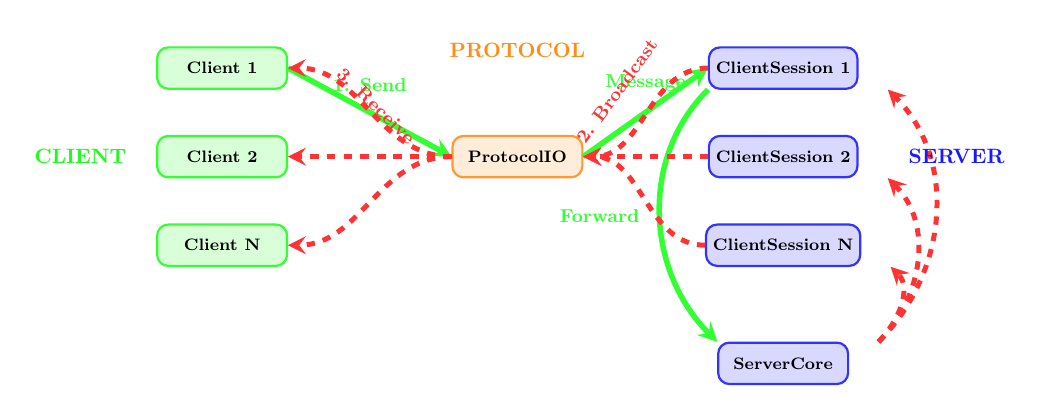
\begin{tikzpicture}[
        scale=0.75,
        transform shape,
        client/.style={rectangle, draw=green!80, fill=green!15, thick, minimum width=2.2cm, minimum height=0.7cm, text centered, font=\footnotesize\bfseries, rounded corners=4pt, align=center},
        server/.style={rectangle, draw=blue!80, fill=blue!15, thick, minimum width=2.2cm, minimum height=0.7cm, text centered, font=\footnotesize\bfseries, rounded corners=4pt, align=center},
        protocol/.style={rectangle, draw=orange!80, fill=orange!15, thick, minimum width=2.2cm, minimum height=0.7cm, text centered, font=\footnotesize\bfseries, rounded corners=4pt, align=center},
        arrow/.style={->, >=stealth, thick, line width=2pt},
        broadcast/.style={->, >=stealth, thick, line width=1.8pt, color=red!80, dashed}
    ]
        
        % ========== CLIENT SIDE (Left) ==========
        \node[client] (client1) at (0,5.5) {Client 1};
        \node[client] (client2) at (0,4) {Client 2};
        \node[client] (clientN) at (0,2.5) {Client N};
        
        % ========== PROTOCOL LAYER (Center) ==========
        \node[protocol] (protocolIO) at (5,4) {ProtocolIO};
        
        % ========== SERVER SIDE (Right) ==========
        \node[server] (clientSession1) at (9.5,5.5) {ClientSession 1};
        \node[server] (clientSession2) at (9.5,4) {ClientSession 2};
        \node[server] (clientSessionN) at (9.5,2.5) {ClientSession N};
        \node[server] (serverCore) at (9.5,0.5) {ServerCore};
        
        % ========== STEP 1: CLIENT SENDS MESSAGE ==========
        \draw[arrow, green!80] (client1.east) -- node[above, font=\small\bfseries, yshift=0.2cm] {1. Send} (protocolIO.west);
        \draw[arrow, green!80] (protocolIO.east) -- node[above, font=\small\bfseries, yshift=0.2cm] {Message} (clientSession1.west);
        % Forward arrow - curved to go around boxes, offset to the left side
        \draw[arrow, green!80] (clientSession1.south west) to[out=225, in=135] node[left, font=\small\bfseries, xshift=-0.2cm] {Forward} (serverCore.north west);
        
        % ========== STEP 2: SERVER BROADCASTS ==========
        % Broadcast arrows - curved to go around boxes, offset further to the right to avoid overlap
        \draw[broadcast] ([xshift=0.5cm]serverCore.north east) to[out=45, in=315] ([xshift=0.5cm]clientSession1.south east);
        \draw[broadcast] ([xshift=0.5cm]serverCore.north east) to[out=45, in=315] ([xshift=0.5cm]clientSession2.south east);
        \draw[broadcast] ([xshift=0.5cm]serverCore.north east) to[out=45, in=315] ([xshift=0.5cm]clientSessionN.south east);
        
        % ========== STEP 3: CLIENTS RECEIVE ==========
        \draw[broadcast] (clientSession1.west) to[out=180, in=0] node[above, font=\small\bfseries, yshift=0.35cm, sloped] {2. Broadcast} (protocolIO.east);
        \draw[broadcast] (clientSession2.west) to[out=180, in=0] (protocolIO.east);
        \draw[broadcast] (clientSessionN.west) to[out=180, in=0] (protocolIO.east);
        
        \draw[broadcast] (protocolIO.west) to[out=180, in=0] node[above, font=\small\bfseries, yshift=-0.1cm, sloped] {3. Receive} (client1.east);
        \draw[broadcast] (protocolIO.west) to[out=180, in=0] (client2.east);
        \draw[broadcast] (protocolIO.west) to[out=180, in=0] (clientN.east);
        
        % ========== LABELS ==========
        \node[font=\normalsize\bfseries, text=green!90, anchor=east] at (-1.5,4) {CLIENT};
        \node[font=\normalsize\bfseries, text=orange!90] at (5,5.8) {PROTOCOL};
        \node[font=\normalsize\bfseries, text=blue!90, anchor=west] at (11.5,4) {SERVER};
        
    \end{tikzpicture}
    \caption{Message Flow Diagram}
    \label{fig:messageflow}
\end{figure}

\section{Whiteboard Drawing Flow}

\begin{enumerate}
    \item User draws on local canvas (mouse drag events)
    \item Client captures stroke coordinates, color, and width
    \item Client sends DRAW\_EVENT message to server
    \item Server broadcasts DRAW\_EVENT to all connected clients
    \item Each client receives and renders the stroke on their canvas
\end{enumerate}

\section{Chat Message Flow}

\begin{enumerate}
    \item User types message and sends
    \item Client creates CHAT message with sender name and text
    \item Server receives and broadcasts to all clients
    \item All clients display message in chat area
    \item Server stores message in history for new connections
\end{enumerate}

\section{File Transfer Flow}

\begin{enumerate}
    \item Sender selects file and target recipients
    \item Client reads file and encodes to Base64
    \item Client sends FILE\_META with file information
    \item Client sends FILE\_CHUNK with encoded data
    \item Client sends FILE\_COMPLETE to signal end
    \item Server routes messages only to selected recipients
    \item Recipients receive file and prompt for save location
    \item File saved with unique identifier suffix
\end{enumerate}

% Section 7: Tools and Technologies
\section{Tools and Technologies}
\label{sec:tools}

\section{Programming Language}

\textbf{Java 25:} The entire project is implemented in Java, providing platform independence and robust networking capabilities through the \texttt{java.net} package.

\section{User Interface Framework}

\textbf{JavaFX 21:} Used for creating the cross-platform graphical user interface. JavaFX provides:
\begin{itemize}
    \item FXML for declarative UI design
    \item Canvas API for whiteboard drawing
    \item Standard controls (MenuBar, ListView, TextArea, etc.)
    \item CSS styling for professional appearance
\end{itemize}

\section{Build Tool}

\textbf{Gradle:} Manages project dependencies, compilation, and execution. Key features:
\begin{itemize}
    \item Platform-specific JavaFX dependency resolution
    \item Custom tasks for server and client execution
    \item Automated build process
\end{itemize}

\section{Libraries}

\begin{itemize}
    \item \textbf{Gson 2.11.0:} JSON serialization and deserialization for protocol messages
    \item \textbf{JavaFX Modules:} javafx-base, javafx-controls, javafx-graphics, javafx-fxml, javafx-swing
\end{itemize}

\section{Development Environment}

\begin{itemize}
    \item Cross-platform development (macOS, Windows, Linux)
    \item Version control: Git
    \item Text editor/IDE: Any Java-compatible IDE
\end{itemize}

\section{Networking}

\begin{itemize}
    \item \textbf{java.net.Socket:} Client-side TCP socket implementation
    \item \textbf{java.net.ServerSocket:} Server-side TCP socket implementation
    \item \textbf{java.io:} Input/output streams for data transmission
\end{itemize}

% Section 8: Applied Networking Concepts
\section{Applied Networking Concepts}
\label{sec:networking}

\section{TCP Socket Programming}

The project extensively uses TCP sockets for all network communication:

\begin{itemize}
    \item \textbf{ServerSocket:} Server creates a \texttt{ServerSocket} listening on port 5050, accepting incoming client connections
    \item \textbf{Socket:} Each client establishes a \texttt{Socket} connection to the server
    \item \textbf{Persistent Connections:} Clients maintain long-lived TCP connections for real-time communication
    \item \textbf{Concurrent Connections:} Server handles multiple clients simultaneously using thread pools
\end{itemize}

\section{Reliable Data Transfer}

The custom protocol ensures reliable data transfer through:

\begin{itemize}
    \item \textbf{Length-prefixed Messages:} Each message begins with a 4-byte integer indicating payload length
    \item \textbf{Complete Message Reading:} Receiver reads exact number of bytes specified in length prefix
    \item \textbf{UTF-8 Encoding:} Consistent character encoding prevents data corruption
    \item \textbf{Connection State Management:} Server tracks connection status and handles disconnections gracefully
\end{itemize}

\section{Message Framing}

To handle TCP's stream nature, messages are framed:

\begin{itemize}
    \item \textbf{Length Prefix:} 4-byte big-endian integer precedes each JSON payload
    \item \textbf{JSON Payload:} Structured data using JSON format for type and content
    \item \textbf{Atomic Reads:} ProtocolIO ensures complete message reading before processing
\end{itemize}

\section{Flow Control}

Flow control is implemented through:

\begin{itemize}
    \item \textbf{Separate Threads:} Reading and writing operations use independent threads to prevent blocking
    \item \textbf{Executor Services:} Thread pools manage concurrent operations efficiently
    \item \textbf{Non-blocking Design:} UI remains responsive while network operations occur in background threads
\end{itemize}

\section{Connection Management}

The server implements connection management:

\begin{itemize}
    \item \textbf{Client Session Tracking:} Each client has a dedicated \texttt{ClientSession} object
    \item \textbf{Connection Lifecycle:} Proper connection establishment, maintenance, and cleanup
    \item \textbf{Error Handling:} Graceful handling of connection failures and client disconnections
    \item \textbf{Broadcast Mechanism:} Efficient message distribution to all connected clients
\end{itemize}

\section{State Synchronization}

State synchronization ensures consistency:

\begin{itemize}
    \item \textbf{History Preservation:} Server maintains chat and drawing history
    \item \textbf{State Transfer:} New clients receive complete state upon connection
    \item \textbf{Event Ordering:} Messages processed in order of receipt
    \item \textbf{Consistent View:} All clients maintain identical whiteboard and chat state
\end{itemize}

\section{Protocol Design}

The custom protocol demonstrates:

\begin{itemize}
    \item \textbf{Message Types:} Enum-based type system for different message categories
    \item \textbf{Structured Payloads:} JSON-based payload structure for flexibility
    \item \textbf{Extensibility:} Easy addition of new message types without breaking existing functionality
\end{itemize}

\section{Congestion Control}

The project implements TCP congestion control algorithms for visualization and educational purposes:

\begin{itemize}
    \item \textbf{TCP Tahoe:} Implements slow start, congestion avoidance, and timeout handling. On 3 duplicate ACKs, drops cwnd to 1 and re-enters slow start.
    \item \textbf{TCP Reno:} Extends Tahoe with fast retransmit and fast recovery. On 3 duplicate ACKs, halves cwnd and enters fast recovery phase.
    \item \textbf{Slow Start:} Exponential growth phase where cwnd increases by 1 for each ACK received, doubling per RTT until reaching ssthresh.
    \item \textbf{Congestion Avoidance:} Linear growth phase where cwnd increases by 1/cwnd per ACK, resulting in 1 packet increase per RTT.
    \item \textbf{Fast Retransmit:} Detection of 3 duplicate ACKs triggers immediate retransmission and congestion response (Reno enters fast recovery, Tahoe re-enters slow start).
    \item \textbf{Fast Recovery:} Reno-specific phase where cwnd is inflated on duplicate ACKs and deflated on new ACK arrival.
    \item \textbf{Timeout Handling:} Both algorithms handle timeout identically by setting ssthresh = cwnd/2, cwnd = 1, and re-entering slow start.
    \item \textbf{RTT Estimation:} Uses exponential weighted moving average (EWMA) to estimate round trip time for timeout calculation.
    \item \textbf{Transmission Round Tracking:} Accurately tracks RTT-based growth by incrementing transmission rounds when full window is acknowledged.
\end{itemize}

% Section 9: Implementation Details
\section{Implementation Details}
\label{sec:implementation}

\section{Project Structure}

The project is organized into three main packages:

\begin{itemize}
    \item \textbf{com.collabwhiteboard.server:} Server-side implementation
    \item \textbf{com.collabwhiteboard.client:} Client-side implementation
    \item \textbf{com.collabwhiteboard.common:} Shared protocol and utilities
\end{itemize}

\section{Server Implementation}

\subsection{ServerCore Class}

\texttt{ServerCore} is the central server component:

\begin{lstlisting}[language=Java, caption=ServerCore Main Loop]
public void run() {
    try (ServerSocket serverSocket = new ServerSocket(port)) {
        while (running) {
            Socket socket = serverSocket.accept();
            int id = clientIdSeq.getAndIncrement();
            ClientSession session = new ClientSession(id, socket, this);
            clients.put(id, session);
            clientPool.submit(session);
            broadcastClientList();
        }
    }
}
\end{lstlisting}

Key responsibilities:
\begin{itemize}
    \item Listens for incoming connections on specified port
    \item Assigns unique client IDs sequentially
    \item Creates \texttt{ClientSession} for each connection
    \item Manages thread pool for concurrent client handling
    \item Maintains client registry and broadcasts updates
\end{itemize}

\subsection{ClientSession Class}

Each \texttt{ClientSession} represents one connected client:

\begin{itemize}
    \item Maintains socket connection and input/output streams
    \item Runs in separate thread for non-blocking operation
    \item Forwards incoming messages to \texttt{ServerCore}
    \item Handles message sending to client
    \item Manages connection lifecycle and cleanup
\end{itemize}

\subsection{Message Routing}

The server routes messages based on type:

\begin{itemize}
    \item \textbf{HELLO:} Updates client display name and sends welcome
    \item \textbf{CHAT, DRAW\_EVENT:} Broadcasts to all clients
    \item \textbf{FILE\_META, FILE\_CHUNK, FILE\_COMPLETE:} Routes to selected recipients
    \item \textbf{CLEAR\_BOARD:} Broadcasts and updates board history
\end{itemize}

\subsection{History Management}

The server maintains two history lists:

\begin{itemize}
    \item \textbf{Chat History:} List of all chat messages with sender and text
    \item \textbf{Board History:} List of all drawing events (strokes)
\end{itemize}

When a new client connects, the server sends:
\begin{itemize}
    \item \texttt{CHAT\_HISTORY} message with all previous chat messages
    \item \texttt{BOARD\_HISTORY} message with all previous drawing events
\end{itemize}

\section{Client Implementation}

\subsection{MainController Class}

\texttt{MainController} manages all client-side functionality:

\begin{itemize}
    \item UI event handling (drawing, chat, file operations)
    \item Network communication with server
    \item Canvas rendering and state management
    \item File handling and user interactions
\end{itemize}

\subsection{Connection Establishment}

\begin{enumerate}
    \item User enters display name (and optional host:port)
    \item Client creates \texttt{Socket} connection to server
    \item Client sends \texttt{HELLO} message with display name
    \item Client receives \texttt{WELCOME} with assigned client ID
    \item Client receives \texttt{CLIENT\_LIST} with current participants
    \item Client receives \texttt{CHAT\_HISTORY} and \texttt{BOARD\_HISTORY}
    \item Client applies history to UI and enters active state
\end{enumerate}

\subsection{Whiteboard Drawing Implementation}

\begin{lstlisting}[language=Java, caption=Drawing Event Handler]
@FXML
private void onCanvasDragged(MouseEvent e) {
    double x = e.getX();
    double y = e.getY();
    Color c = colorPicker.getValue();
    double stroke = strokeSlider.getValue();
    
    // Draw locally
    gc.setStroke(c);
    gc.setLineWidth(stroke);
    gc.strokeLine(lastX, lastY, x, y);
    
    // Send to server
    JsonObject payload = new JsonObject();
    payload.addProperty("x1", lastX);
    payload.addProperty("y1", lastY);
    payload.addProperty("x2", x);
    payload.addProperty("y2", y);
    payload.addProperty("color", toWebColor(c));
    payload.addProperty("stroke", stroke);
    sendAsync(new ProtocolMessage(MessageTypes.DRAW_EVENT, payload));
    
    lastX = x;
    lastY = y;
}
\end{lstlisting}

\subsection{Chat Implementation}

Chat messages are sent asynchronously:

\begin{enumerate}
    \item User types message and presses Enter or clicks Send
    \item Client creates \texttt{CHAT} message with display name and text
    \item Message sent to server via \texttt{sendAsync}
    \item Server broadcasts to all clients
    \item All clients receive and display in chat area
\end{enumerate}

\subsection{File Transfer Implementation}

File transfer uses a three-phase protocol:

\begin{enumerate}
    \item \textbf{FILE\_META:} Sends file name, size, unique ID, and target recipient IDs
    \item \textbf{FILE\_CHUNK:} Sends Base64-encoded file data
    \item \textbf{FILE\_COMPLETE:} Signals end of transfer
\end{enumerate}

Recipients:
\begin{enumerate}
    \item Receive \texttt{FILE\_META} and initialize buffer
    \item Receive \texttt{FILE\_CHUNK} and append to buffer
    \item Receive \texttt{FILE\_COMPLETE} and prompt for save location
    \item Save file with unique identifier suffix
\end{enumerate}

\section{Protocol Implementation}

\subsection{ProtocolIO Class}

\texttt{ProtocolIO} handles low-level message transmission:

\begin{itemize}
    \item \textbf{sendMessage:} Serializes message to JSON, writes length prefix, then payload
    \item \textbf{readMessage:} Reads length prefix, then reads exact number of bytes, parses JSON
    \item Uses \texttt{DataInputStream} and \texttt{DataOutputStream} for binary operations
\end{itemize}

\subsection{Message Format}

Each message consists of:
\begin{itemize}
    \item 4-byte integer (big-endian): JSON payload length
    \item UTF-8 JSON string: \texttt{\{"type": "MESSAGE\_TYPE", "payload": \{...\}\}}
\end{itemize}

\subsection{Threading Model}

\begin{itemize}
    \item \textbf{Server:} Uses \texttt{ExecutorService} thread pool for client sessions
    \item \textbf{Client:} Separate executors for reading (blocking) and sending (non-blocking)
    \item Prevents UI freezing and ensures responsive user experience
\end{itemize}

\section{UI Implementation}

\subsection{FXML Layout}

The UI is defined in \texttt{MainView.fxml}:

\begin{itemize}
    \item \texttt{BorderPane} as root container
    \item \texttt{MenuBar} at top for File and Board menus
    \item \texttt{SplitPane} for whiteboard and chat areas
    \item \texttt{Canvas} for drawing surface
    \item \texttt{ListView} for connected clients
    \item \texttt{TextArea} for chat display
\end{itemize}

\subsection{CSS Styling}

Custom stylesheet (\texttt{app.css}) provides:
\begin{itemize}
    \item Professional color scheme
    \item Rounded buttons and modern appearance
    \item Consistent menu styling
    \item Cross-platform compatible design
\end{itemize}

\section{Congestion Control Implementation}

\subsection{CongestionController Class}

The \texttt{CongestionController} class implements the core congestion control algorithms:

\begin{itemize}
    \item \textbf{Initialization:} Sets initial cwnd=1, ssthresh=64, phase=SLOW\_START
    \item \textbf{onAckReceived:} Main logic for handling ACKs, updating cwnd based on current phase and algorithm mode
    \item \textbf{onTimeout:} Handles timeout events by resetting cwnd to 1 and ssthresh to cwnd/2
    \item \textbf{handleFastRetransmit:} Reno-specific fast retransmit logic triggered on 3 duplicate ACKs
    \item \textbf{updateRTT:} Updates estimated RTT using EWMA formula: \texttt{estimatedRTT = 0.875 * oldRTT + 0.125 * sampleRTT}
    \item \textbf{Transmission Round Tracking:} Increments transmission round when ACKs for full window are received
\end{itemize}

\subsection{CongestionAwareProtocolIO Class}

This class provides a client-side simulation layer:

\begin{itemize}
    \item \textbf{Packet Simulation:} Splits messages into simulated packets based on MSS (1460 bytes)
    \item \textbf{ACK Simulation:} Generates ACKs for successfully transmitted packets after network delay
    \item \textbf{Timeout Detection:} Monitors unacknowledged packets and triggers timeout when age exceeds 2*RTT
    \item \textbf{Packet Loss Simulation:} Applies configurable packet loss rate to simulate network conditions
    \item \textbf{Network Delay:} Simulates network latency with configurable delay parameter
    \item \textbf{Backward Compatibility:} Messages are still sent via regular ProtocolIO, maintaining compatibility
\end{itemize}

\subsection{UI Integration}

The congestion control UI is integrated into the main application:

\begin{itemize}
    \item \textbf{TabPane Layout:} Congestion control panel accessible via dedicated tab alongside client list
    \item \textbf{Real-time Updates:} Metrics and graph update automatically on state changes
    \item \textbf{Interactive Controls:} Toggle button to enable/disable, radio buttons for algorithm selection
    \item \textbf{Graph Visualization:} LineChart displays cwnd vs transmission rounds with auto-scaling axes
    \item \textbf{Activity Log:} TextArea displays chronological log of congestion control events
\end{itemize}

\subsection{Algorithm Accuracy}

The implementation accurately follows TCP Tahoe and Reno specifications:

\begin{itemize}
    \item \textbf{Slow Start:} cwnd += 1 per ACK (exponential growth)
    \item \textbf{Congestion Avoidance:} cwnd += 1/cwnd per ACK using fractional counter (linear growth)
    \item \textbf{ssthresh Behavior:} Only decreases on congestion events, never increases
    \item \textbf{Tahoe on 3 Duplicate ACKs:} ssthresh = cwnd/2, cwnd = 1, re-enter slow start
    \item \textbf{Reno on 3 Duplicate ACKs:} ssthresh = cwnd/2, cwnd = ssthresh, enter fast recovery
    \item \textbf{Fast Recovery:} cwnd += 1 per duplicate ACK, exit on new ACK
\end{itemize}

% Section 10: Result Analysis
\section{Result Analysis}
\label{sec:results}

\section{Application Screenshots}

\subsection{Server Startup}

\begin{figure}[H]
    \centering
    \includegraphics[width=0.8\textwidth]{screenshots/server_startup.png}
    \caption{Server successfully started and listening on port 5050}
    \label{fig:server_startup}
\end{figure}

The server initializes and begins listening for client connections. The console output confirms the server is ready to accept connections.

\subsection{Client Connection}

\begin{figure}[H]
    \centering
    \includegraphics[width=0.8\textwidth]{screenshots/client_connection.png}
    \caption{Client connection dialog and successful connection}
    \label{fig:client_connection}
\end{figure}

Clients can connect by entering a display name. The status bar shows connection confirmation with assigned client ID.

\subsection{Multi-Client Whiteboard}

\begin{figure}[H]
    \centering
    \includegraphics[width=0.9\textwidth]{screenshots/multi_client_whiteboard.png}
    \caption{Multiple clients drawing simultaneously with synchronized strokes}
    \label{fig:multi_client}
\end{figure}

This screenshot demonstrates real-time collaboration with multiple clients. Strokes drawn by one client appear immediately on all other clients' whiteboards, demonstrating successful synchronization.

\subsection{Chat Functionality}

\begin{figure}[H]
    \centering
    \includegraphics[width=0.8\textwidth]{screenshots/chat_functionality.png}
    \caption{Chat messages synchronized across all clients}
    \label{fig:chat}
\end{figure}

The chat system successfully broadcasts messages to all connected clients. Message history is preserved and displayed to newly connected clients.

\subsection{File Sharing}

\begin{figure}[H]
    \centering
    \includegraphics[width=0.8\textwidth]{screenshots/file_sharing.png}
    \caption{File sharing with recipient selection and unique file naming}
    \label{fig:file_sharing}
\end{figure}

\begin{figure}[H]
    \centering
    \includegraphics[width=0.8\textwidth]{screenshots/sender_send.png}
    \caption{File sharing notification for sender side}
    
\end{figure}

\begin{figure}[H]
    \centering
    \includegraphics[width=0.8\textwidth]{screenshots/receiver_receive.png}
    \caption{File sharing notification for receiver side}
    
\end{figure}



The file sharing feature allows selective recipient targeting. Received files are automatically renamed with unique identifiers as shown in the save dialog.

\subsection{Client List}

\begin{figure}[H]
    \centering
    \includegraphics[width=0.6\textwidth]{screenshots/client_list.png}
    \caption{Dynamic client list showing all connected participants}
    \label{fig:client_list}
\end{figure}

The client list dynamically updates as clients connect and disconnect, showing all active participants with their assigned IDs.

\subsection{Congestion Control Visualization}

\begin{figure}[H]
    \centering
    \includegraphics[width=0.9\textwidth]{screenshots/congestion_control.png}
    \caption{TCP Congestion Control visualization showing real-time metrics, graph, and activity log}
    \label{fig:congestion_control}
\end{figure}

The congestion control panel provides comprehensive visualization of TCP Tahoe and Reno algorithms. The screenshot shows:
\begin{itemize}
    \item Real-time metrics display (cwnd, ssthresh, RTT, phase)
    \item Interactive graph showing cwnd evolution over transmission rounds
    \item Network simulation controls (packet loss rate and delay sliders)
    \item Activity log displaying congestion control events
    \item Algorithm selection (Tahoe/Reno) and enable/disable toggle
\end{itemize}

The graph clearly demonstrates the different phases of congestion control: exponential growth during slow start, linear growth during congestion avoidance, and recovery events (timeout or fast retransmit).

\subsection{Cross-Platform Compatibility}

\begin{figure}[H]
    \centering
    \begin{subfigure}{0.45\textwidth}
        \includegraphics[width=\textwidth]{screenshots/windows_ui.png}
        \caption{Windows}
    \end{subfigure}
    \hfill
    \begin{subfigure}{0.45\textwidth}
        \includegraphics[width=\textwidth]{screenshots/macos_ui.png}
        \caption{macOS}
    \end{subfigure}
    \caption{Consistent UI across different operating systems}
    \label{fig:cross_platform}
\end{figure}

The application maintains identical functionality and appearance across Windows, macOS, and Linux platforms, demonstrating successful cross-platform implementation.

\section{Performance Analysis}

\begin{itemize}
    \item \textbf{Latency:} Drawing events appear on other clients within milliseconds
    \item \textbf{Throughput:} Server handles multiple concurrent clients without performance degradation
    \item \textbf{Reliability:} Connection failures handled gracefully with proper cleanup
    \item \textbf{Memory:} Efficient message handling prevents memory leaks
\end{itemize}

\section{Testing Scenarios}

\begin{enumerate}
    \item \textbf{Single Client:} Verified basic functionality with one client
    \item \textbf{Multiple Clients:} Tested with 2-5 simultaneous clients
    \item \textbf{History Synchronization:} Confirmed new clients receive complete state
    \item \textbf{File Transfer:} Verified file integrity and unique naming
    \item \textbf{Cross-Platform:} Tested on Windows, macOS, and Linux
    \item \textbf{Network Disconnection:} Confirmed graceful handling of connection failures
\end{enumerate}

% Section 11: Summary
\section{Summary of the Project}
\label{sec:summary}

This project successfully implements a collaborative whiteboard and file sharing application using pure TCP protocol, demonstrating practical application of networking concepts learned throughout the course. The system provides real-time collaboration capabilities with synchronized whiteboard drawing, integrated chat, and secure file transfer functionality.

The implementation showcases several key achievements:

\begin{itemize}
    \item \textbf{Protocol Design:} Custom TCP-based protocol with length-prefixed message framing ensures reliable data transfer
    \item \textbf{Architecture:} Client-server model with centralized state management enables scalable multi-user collaboration
    \item \textbf{Cross-Platform:} Single codebase functions identically on Windows, macOS, and Linux
    \item \textbf{User Experience:} Professional UI with responsive interactions and intuitive controls
    \item \textbf{Reliability:} Robust error handling and connection management ensure stable operation
    \item \textbf{Congestion Control:} Accurate implementation of TCP Tahoe and Reno algorithms with real-time visualization demonstrates deep understanding of network congestion management
\end{itemize}

The project successfully addresses all design objectives, providing a functional collaborative tool that demonstrates deep understanding of TCP socket programming, protocol design, and concurrent network application development. The implementation serves as a practical example of how networking concepts can be applied to create real-world collaborative applications.

% Section 12: Limitations and Future Plan
\section{Limitations and Future Plan}
\label{sec:limitations}

\section{Current Limitations}

\begin{enumerate}
    \item \textbf{Scalability:} The current implementation may face performance issues with a very large number of concurrent clients (100+). The server uses a simple broadcast mechanism that sends messages to all clients regardless of relevance.
    
    \item \textbf{No Authentication:} The system lacks user authentication and authorization mechanisms. Any client can connect with any display name without verification.
    
    \item \textbf{No Encryption:} All data transmission occurs in plain text. Sensitive information could be intercepted on untrusted networks.
    
    \item \textbf{No Persistence:} Server state (chat history, board history) is maintained only in memory. Server restart results in complete data loss.
    
    \item \textbf{Limited File Size:} Large file transfers may cause memory issues as entire files are loaded into memory before transmission.
    
    \item \textbf{No Undo/Redo:} The whiteboard lacks undo/redo functionality for drawing operations.
    
    \item \textbf{No Drawing Tools:} Only freehand drawing is supported. Shapes, text, and other drawing tools are not available.
    
    \item \textbf{Single Server:} No support for multiple servers or server clustering for high availability.
    
    \item \textbf{Congestion Control Simulation:} The congestion control implementation is a client-side simulation for visualization purposes and doesn't affect actual TCP protocol behavior.
\end{enumerate}

\section{Future Enhancements}

\subsection{Short-term Improvements}

\begin{itemize}
    \item \textbf{User Authentication:} Implement login system with username/password or token-based authentication
    \item \textbf{Encryption:} Add TLS/SSL support for encrypted communication
    \item \textbf{Undo/Redo:} Implement drawing history with undo/redo capabilities
    \item \textbf{Drawing Tools:} Add shapes (rectangle, circle, line), text tool, and eraser
    \item \textbf{File Size Limits:} Implement chunked file transfer for large files
    \item \textbf{Database Integration:} Store chat and board history in database for persistence
\end{itemize}

\subsection{Long-term Enhancements}

\begin{itemize}
    \item \textbf{Server Clustering:} Implement distributed server architecture for horizontal scaling
    \item \textbf{Message Queuing:} Use message queue system for better scalability and reliability
    \item \textbf{Web Client:} Develop web-based client using WebSocket (while maintaining TCP for desktop clients)
    \item \textbf{Mobile Support:} Create mobile applications for iOS and Android
    \item \textbf{Advanced Features:} 
    \begin{itemize}
        \item Voice/video chat integration
        \item Screen sharing capabilities
        \item Collaborative document editing
        \item Version control for whiteboard states
    \end{itemize}
    \item \textbf{Analytics:} Implement usage analytics and monitoring dashboard
    \item \textbf{Cloud Deployment:} Deploy server infrastructure on cloud platforms with auto-scaling
\end{itemize}

\section{Technical Improvements}

\begin{itemize}
    \item \textbf{Protocol Optimization:} Implement message compression to reduce bandwidth usage
    \item \textbf{Connection Pooling:} Optimize connection management for better resource utilization
    \item \textbf{Caching:} Implement caching mechanisms for frequently accessed data
    \item \textbf{Load Balancing:} Add load balancing support for multiple server instances
    \item \textbf{Monitoring:} Integrate logging and monitoring tools for production deployment
\end{itemize}

\end{document}

